\chapter{Theoretische Grundlagen}
\label{chap:theorie}

\section{Geschichte der Neutrinos}
\label{sec:neutrinogeschichte}

Neutrinos wurden erstmals am $4.$ Dezember $1930$ von Pauli als Spin-$\frac{1}{2}$-Teilchen postuliert, um das Problem der Drehimpulserhaltung und das kontinuierliche Elektronenspektrum beim $\beta$-Zerfall zu lösen. %\cite{zuber}
Er führte das Neutrino als Teilchen ein, dass beim $\beta^-$-Zerfall
\begin{equation*}
    n \rightarrow p + e^- + \bar{\nu}_e
\end{equation*}
gemeinsam mit dem Elektron emittiert wird, anders als dieses allerdings nicht detektierbar ist. \\
Diese Annahme Paulis wurde lange kritisch betrachtet, bis Neutrinos in den $50$er Jahren in Atomreaktoren zweifellos nachgewiesen werden konnten. %\cite{zuber}\\

Im Standardmodell der Teilchen sind Neutrinos als einzige masselose, elektrisch neutrale Leptonen vertreten.
Theoretisch lassen sie die Wellenfunktionen $\psi$, als lorentzinvariante Lösung der relativistischen Diracgleichung
\begin{equation}
    \left(i \gamma_\mu \frac{\partial}{\partial x_\mu} - m \right) \psi = 0
    \label{eq:dirac}
\end{equation}
beschreiben.
Die Wellenfunktion ist dabei ein vierkomponentiger Spinor, $\gamma_\mu$ sind die $4 \times 4$-Diracmatrizen der Darstellung
\begin{align}
    \gamma_0 = \left( \begin{array}{c c}
        \mathbb{1} & 0          \\ 
        0          & -\mathbb{1} \\ 
        \end{array}\right) \,,
    &&
    \gamma_k = \left( \begin{array}{c c}
        0           & \sigma_k  \\ 
        -\sigma_k   & 0         \\ 
        \end{array}\right) \,,
    \label{eq:gammamatrizen}
\end{align}
wobei $\mathbb{1}$ die Einheitsmatrix und $\sigma_k$ mit $k = 1, 2, 3$ die $2 \times 2$-Paulimatrizen
\begin{align}
    \sigma_1 = \left( \begin{array}{c c}
        0 & 1   \\ 
        1 & 0   \\ 
        \end{array}\right) \,,
    &&
    \sigma_2 = \left( \begin{array}{c c}
        0           & -i  \\ 
        i  & 0         \\ 
        \end{array}\right) \,,
    &&
    \sigma_3 = \left( \begin{array}{c c}
        1           & 0 \\ 
        0   & -1         \\ 
        \end{array}\right)
\end{align}
darstellen. 

Somit sind Neutrinos auch die einzigen Leptonen, die nicht nur nicht stark wechselwirken, sondern auch nicht an der schwachen Wechselwirkung teilnehmen.
Tatsächlich ist ihre Wechselwirkung mit Materie so gering, dass die $7 \cdot 10^{10}$  Neutrinos, die pro $\si{\centi\meter}^2$ und pro Sekunde auf die Erde treffen, keinerlei Auswirkung
auf das Leben ihrer Bewohner haben \cite[S. ~133]{grupen}. 

Zu jeder der drei Leptonengenerationen, sprich Elektronen, Myonen und Tauonen existiert dabei ein korrespondierendes Neutrino.
Dieser sogenannte Flavour eines Neutrinos ist dabei nicht fest, sondern kann sich zeitlich und räumlich periodisch ändern.
Die Entdeckung dieser sogenannten Neutrinooszillationen erhielt im Jahre $2015$ den Nobelpreis \cite[S. ~19]{oberauer}.


\section{Neutrinos in verschiedenen Basen}
\label{sec:neutrinobasen}

\subsection{Flavourbasis} %\cite[Kap. 2.1]{oberauer}
\label{subsec:flavourbasis}
Voraussetzung für die Neutrinooszillationen ist aber, dass Masseneigenzustände $\nu_i$ als Lösungen der Diracgleichung mit den Masseneigenwerten $m_i (i = 1, 2, 3)$ existieren.
Diese Masseneigenzustände bestimmen die Propagation des Neutrinos im Vakuum und müssen nicht zwangsläufig identisch zu den Flavoureigenzuständen sein.
Hier betrachten wir die Flavoureigenzustände $\nu_\alpha (\alpha = e, \mu, \tau)$ als Superposition der Masseneigenzustände mit
\begin{equation}
    \nu_\alpha = \sum_i U_{\alpha i} \nu^{(h_i)}_i \,,
    \label{eq:flavourbasis}
\end{equation}
wobei $U_{\alpha i}$ die unitäre Pontecorvo-Maki-Nakagawa-Sakata-Mischungsmatrix (PMNS-Matrix) zwischen Massenbasis und Flavourbasis darstellt und eine Aussage über die Wahrscheinlichkeit der Oszillation zwischen bestimmten Eigenzuständen macht.
Das Superskript $(h_i) = \pm 1$ beschreibt dabei die Helizität des Eigenzustands und ist hier nicht weiter von Relevanz.


\subsection{Materiebasis} %\cite{päspaper}
\label{subsec:materiebasis}

Zur Beschreibung der Propagation von Neutrinos in besonders dichten Medien wird eine weitere Basis, die Materiebasis genutzt.
Die Materieeigenzustände
\begin{equation}
    \tilde{\nu}^{(h_i)}_i = \sum_i \tilde{U}_{i j} \nu^{(h_j)}_j
    \label{eq:materiebasis}
\end{equation} lassen sich, ähnlich wie die Flavoureigenzustände, ebenfalls als Superposition der Masseneigenzustände beschreiben, lediglich die Mischungsmatrix unterscheidet sich.


\section{Neutrinos und spontane Symmetriebrechung}

Um die Masse der Neutrinos zu erklären, führen wir ein Quantenfeld ein, das Majoronenfeld, welches die Leptonenzahlsymmetrie, wenn auch nur geringfügig, bricht.
Dazu sollen hier zunächst einige Begrifflichkeiten geklärt werden.

\subsection{Das Eichprinzip} %\cite{kleingrot}

Das Prinzip der Eichinvarianz beschreibt Transformationen, die die Physik eines Systems, also die Lagrangedichte, invariant lassen.
Dabei unterscheiden wir zwischen globalen Transformationen, die sich, unabhängig von Raum und Zeit, überall gleichartig auf das System auswirken und lokalen Eichtransformationen, 
die von Ort und Zeit abhängig unterschiedlich auf das System wirken.

Für uns sind im Folgenden insbesondere die globalen Symmetrien relevant.
Jede dieser globalen Symmetrien, ist durch das Noether-Theorem mit einer Erhaltungsgröße verknüpft.
Unter globale Transformationen fallen beispielsweise die Multiplikation der Lösung $\psi$ der Schrödingergleichung um eine konstante komplexe Phase $\mathrm{e}^{i \alpha}$.

\subsection{Spontane Symmetriebrechung} %\cite{kleingrot}


Der Mechanismus der spontanen Symmetriebrechung erlaubt uns, massebehaftete Eichbosonen einzuführen, ohne die Eichinvarianz der Lagrangedichte durch explizite Massenterme zu verlieren.
Konkret sprechen wir von einer spontanen Symmetriebrechung, wenn die grundlegenden Gleichungen eines Systems über eine Symmetrie verfügen, der der Grundzustand nicht folgt.

Das Majoronenfeld, also auch die dazugehörigen Eichbosonen, die Majoronen, lässt sich durch ein Potential einführen, dessen Vakuumerwartungswert (VEV), also der Zustand niedrigster Energie $E_\text{min}$ entartet. \\
Wir fordern also, dass unser System, beschrieben durch den Hamiltonian $H$, invariant unter einer Transformation $U$ bleibt, sprich der Kommutator $[H, U]$ verschwindet.
Es gilt also auch
\begin{equation*}
    H U \ket{0} = U H \ket{0} = E_\text{min} U  \ket{0} 
\end{equation*}
und damit
\begin{equation*}
    U \ket{0}_i = \ket{0}_j \,, \quad i \neq j \,,
\end{equation*}
sofern mehrere entartete Zustände $\ket{0}_i$ existieren. \\
Die Transformation $U$ lässt das Vakuum $\ket{0}$ also nicht notwendigerweise invariant.

Das einfachste Potential mit diesen Eigenschaften besitzt die Form
\begin{equation}
    V(x) = -\frac{1}{2} \mu^2 x^2 + \frac{1}{4} \lambda x^4 \,, \quad \mu,\lambda > 0 \,.
\end{equation}
Offensichtlich ist dieses, auch Mexico-Hut-Potential genannte, Potential radialsymmetrisch.
Es existiert also ein Kreis mit Radius
\begin{equation*}
    x_0 = \sqrt{\frac{\mu^2}{\lambda}} \,,
\end{equation*}
auf dem die Zustände minimaler Energie verteilt sind.
\autoref{fig:mexicohutpot} zeigt eine Darstellung des Potentials in zwei Dimensionen.

\begin{figure}
    \centering
    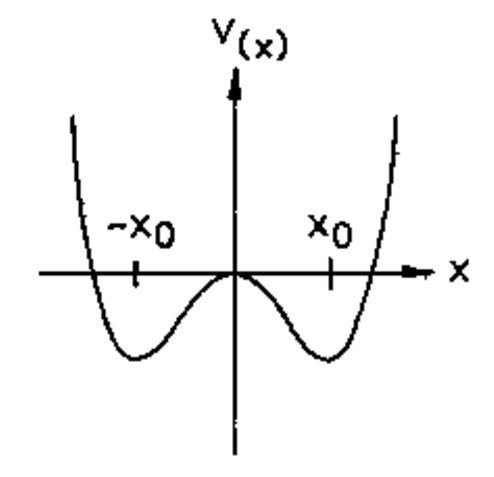
\includegraphics[]{figures/MexicoHutpotential.pdf}
    \caption{Darstellung des Mexico-Hut-Potentials in zwei Dimensionen. Zu erkennen sind die zwei möglichen Grundzustände $x = \pm x_0$ \cite{kleingrot}.}
    \label{fig:mexicohutpot}
\end{figure}

Anschaulich stellen wir uns vor, dass wir uns zunächst im Zentrum des Potentials befinden.
Von diesem Punkt aus besitzt das Potential eine globale Symmetrie, egal in welche Richtung wir schauen.
Betrachten wir das ganze aber von einem der Vakua, existiert diese Symmetrie unter der Transformation $x \rightarrow -x$ nicht länger.



\section{Einfluss von Majoronen auf Supernovaexplosionen}

